\subsection{End to End Device Test}

The test showed that, with the increased Hough space resolution, the device was 
able to detect when the perch came in range and close around it. A video of the 
process was captured, screenshots from it are shown in Fig. \ref{fig:e2e-vid}.

The device was very slow to detect the perch, with a delay of 93 seconds % in range at 0:07, closed at 1:40
between the perch being moved into range and the device detecting it and closing the grasper over it. 

\begin{figure}[H]
    \centering
    % Generated from "C:\Users\wyatt\Documents\GVSU\Thesis\prototype testing\test bin files\test_7"
    \begin{subfigure}[b]{\textwidth}        
        \begin{subfigure}[b]{\textwidth}
            \centering
            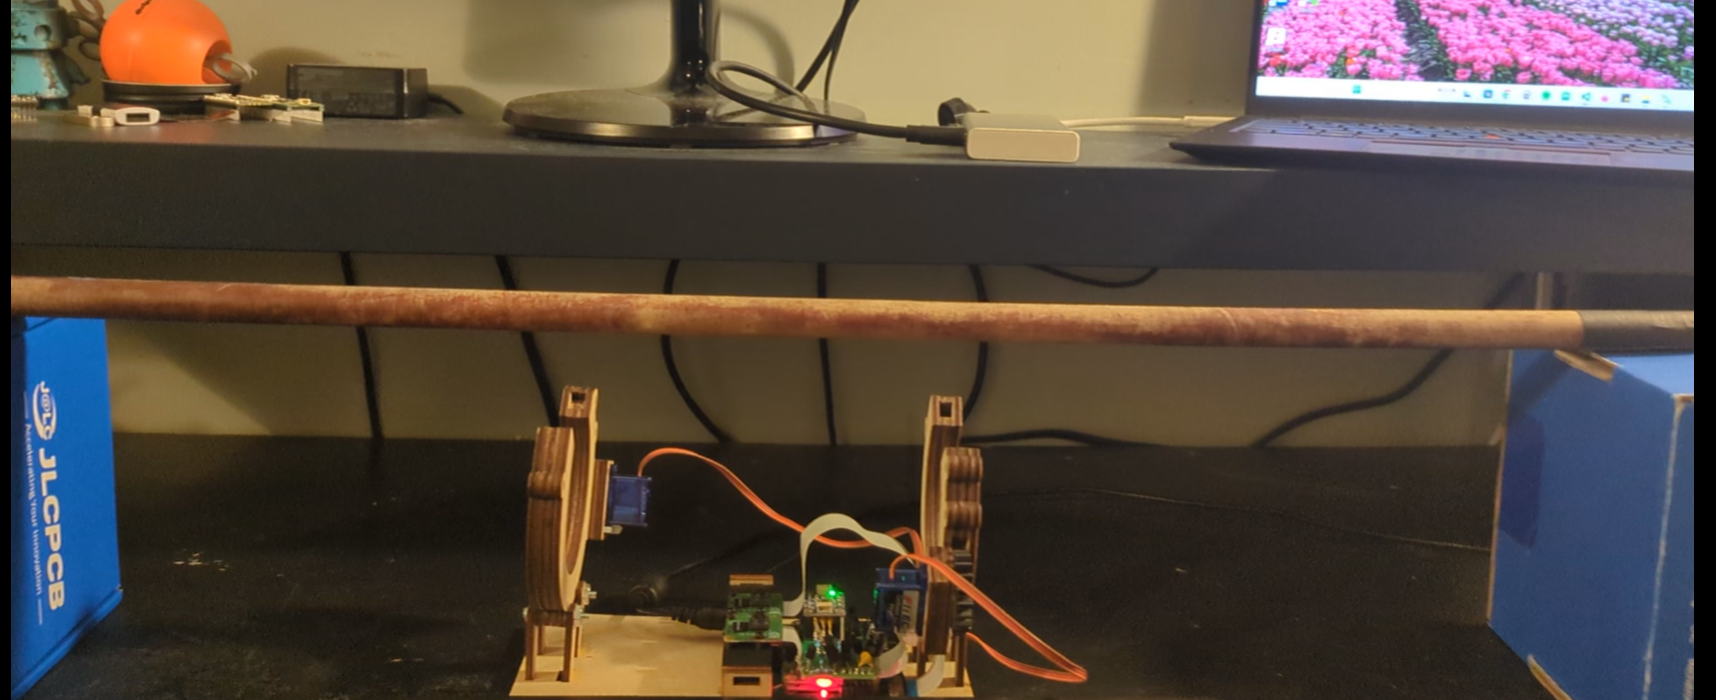
\includegraphics[width=\textwidth]{sections/results/e2e-vid-1.png}
            \caption{The start of the test, with the perch out of range.}
            \label{fig:e2e-vid:3}
        \end{subfigure}
        \vfill
        \begin{subfigure}[b]{\textwidth}
            \centering
            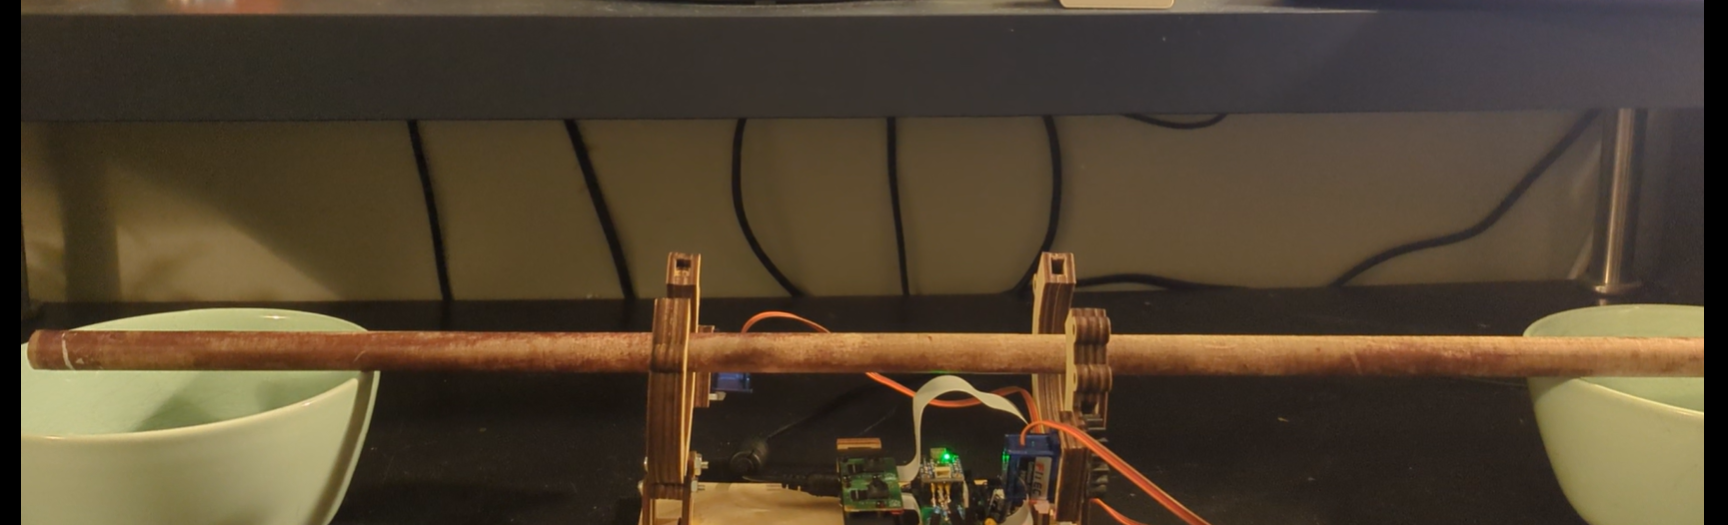
\includegraphics[width=\textwidth]{sections/results/e2e-vid-2.png}
            \caption{The middle of the test, with the perch moved into range.}
            \label{fig:e2e-vid:3}
        \end{subfigure}
        \vfill
        \begin{subfigure}[b]{\textwidth}
            \centering
            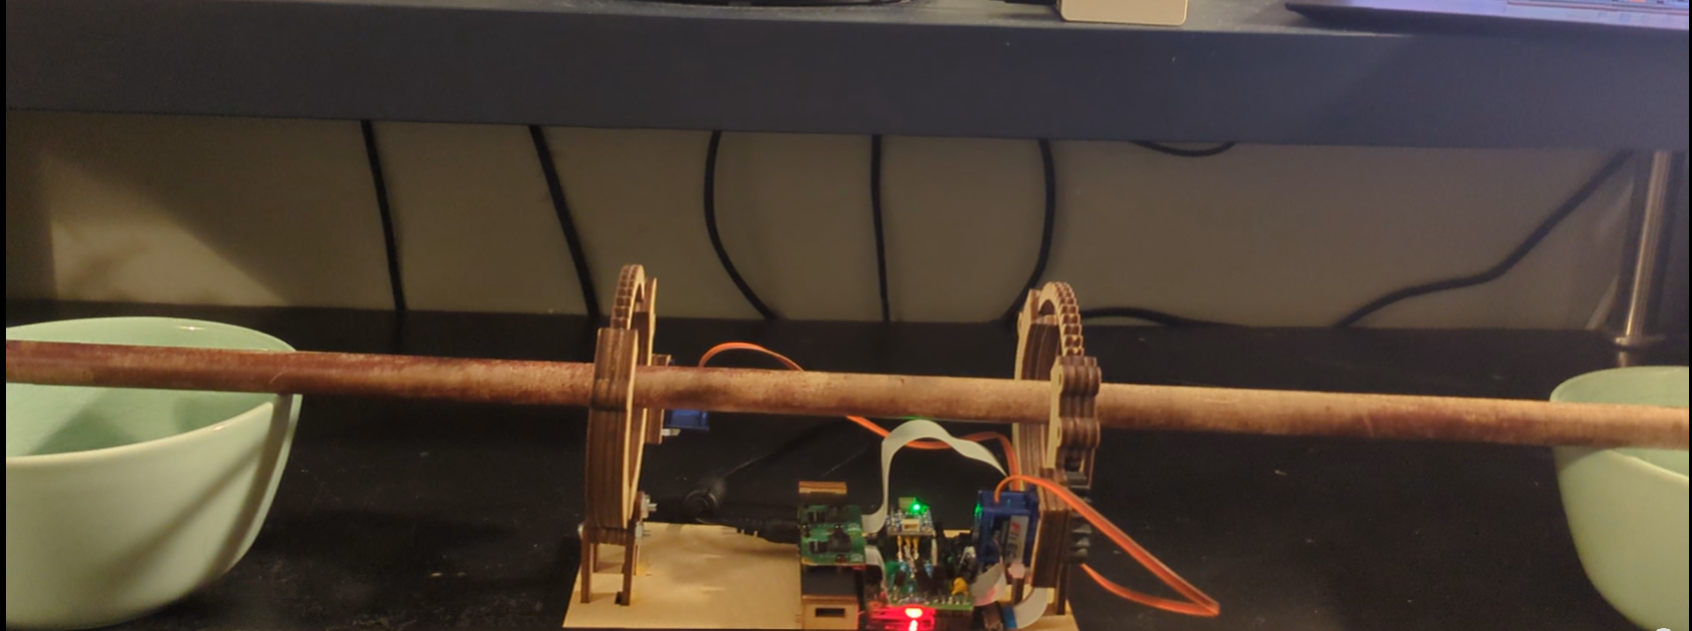
\includegraphics[width=\textwidth]{sections/results/e2e-vid-3.png}
            \caption{The end of the test, with the perch in range and the grasper closed over it.}
            \label{fig:e2e-vid:3}
        \end{subfigure}
    \end{subfigure}
    \caption{Screenshots from the video of the device successfully detecting and grasping around a perch.}
    \label{fig:e2e-vid}
\end{figure}